\documentclass{article}
\usepackage[utf8]{inputenc}
\documentclass{aastex63}
\newcommand{\vdag}{(v)^\dagger}
\newcommand\aastex{AAS\TeX}
\newcommand\latex{La\TeX}
\newcommand{\vdag}{(v)^\dagger}
\newcommand\aastex{AAS\TeX}
\newcommand\latex{La\TeX}

\title{Research Assignment 2}
\author{Adrien Masini }
\date{March 2020}

\documentclass{article}
\usepackage{graphicx}
\graphicspath{ {./images/} }

\begin{document}
\maketitle
\section{Introduction}


- We are going to study the behavior of the dark matter halo of M33 due to tidal forces caused by MW and M31 and later by the MW-M31 merger. M33 is a spiral galaxy, third member of the local group with the Milky Way (MW) and Andromeda (M31). It is believed that M33 is a satellite of M31. In detail, we will observe and map the evolution of M33's dark matter halo when it will be orbiting the MW-M31 system. Also, we will study how dark matter profile evolves due to mass loss from tides and quantify the mass loss rate as a function of time.
\vspace{0.5mm}

Dark matter seems to play an important in galaxy formation and  evolution due to collisions. Dark matter structures merge to form bigger structures, but as they merge, the smaller halo is not necessarily absorbed immediately and can become a sub-halo of the all structure \cite{Delos19}. By studying dark matter halo due to tidal forces, we will be able to understand the physics behind how galaxies formed.
\vspace{0.5mm}

We know almost nothing about the behavior of Dark Matter except that even though we cannot see it, it interacts with normal matter via gravity. That property will allow us to predict the behavior of Dark Matter structure as the galaxies and halos merge during a collision using a simulation.
\vspace{0.5mm}

An important question in the field is questioning how does normal matter behave due to the physical properties of dark matter \cite{Wechsler18} and scientists think that the Baryonic matter has a direct impact in the density profile of dark matter halo \cite{Grillo12}.
\vspace{5mm}

Figure 1 below show the density profile of a Dark Matter Halo or a simulated galaxy as a function of radius at different time. This study did not take into account the dynamical friction between  the small sub-halo and the larger halo that merged together. This approximation is correct as long as the ratio of the mass is of the order of a hundred (M/m = 100) which is right for our MW-M31 halo system compared to the M33 sub-halo.


\begin{figure}[htp]
    \centering
    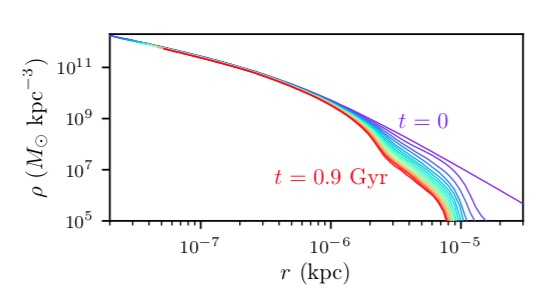
\includegraphics[width=7cm]{DensityProfileEvolutionOfHalo.jpeg}
    \caption{\cite{Delos19} Density Profile Evolution Of Halo}
    \label{fig:galaxy}
\end{figure}

\vspace{5mm}
\vspace{5mm}
\vspace{5mm}

\vspace{5mm}
\vspace{5mm}
\vspace{5mm}
\maketitle
\section{Proposal :}
\vspace{5mm}

In this research, we will be answering the following questions :
\vspace{0.5mm}

    - How does dark matter halo evolve over time due to the tidal forces from a collision of galaxies ?
\vspace{0.5mm}    

To answer that question we will use the data we have on halo particles for M33 and MW-M31 and track how the density profile of M33's Dark matter halo evolve over time using a plot of density profile over time. We will need to use the center of mass class we created to keep track of the galaxies position and velocities.
\vspace{0.5mm}

I think the density of the halo should decrease until M33 collides with the new MW-M31 merger system and then the two halos will add their own Dark Matter to form a new more massive halo of Dark Matter.










\bibliography{citation}{}
\bibliographystyle{aasjournal}

\end{document}
